\section{Sécurisation du drone}
Comme nous avons pu le voir, cet ARDrone 2.0 de \textbf{Parrot} rencontre de nombreux problèmes de sécurité et reste vulnérable à certaines attaques. L'une des vulnérabilités principales se trouve dans le point d'accès Wifi qui est un réseau ouvert donc accessible à toute personne se trouvant à portée du drone.

\subsection{Sécurisation via le Wifi}
\paragraph{Modification du point d'accès}
L'une des premières mesures pour ce drone serait donc une modification de ce point d'accès Wifi en y ajoutant un mot de passe afin de le rendre privé. Afin de minimiser les risques de compromission du réseau, l'utilisation de la norme WPA2 semble optimale. Après un rapide état de l'art sur Internet, il semblerait que personne ne se soit réellement penché sur le problème mais un fichier bash présent sur le drone, \textit{wifi\_setup.sh}, laisse présager que cette modification est possible. On peut aussi noter que les nouveaux drone de la société Parrot possèdent une meilleure sécurité au niveau du Wifi. En effet, le Bebop propose un Wifi WPA2 avec mot de passe mais ce n'est pas la configuration par défault.

\paragraph{Utilisation du drone comme un client}
Une autre solution consisterait à utiliser le drone non comme un point d'accès mais comme un client du Wifi.
Afin de pouvoir connecter le drone à un réseau en WPA2, il est nécessaire d'effectuer de la compilation croisée sur le module \textit{wpa\_supplicant}, qui gère les connections au wifi WPA2 sur les environements Unix. En effet, le drone possède une architecture ARM et non x86. Heureusement, la communauté est riche de talent, et ce travail a déjà été fait dans ce dépot Github: \url{https://github.com/daraosn/ardrone-wpa2}.\cite{ref7}\\

Cette manipulation se fait en plusieurs étapes:
\begin{itemize}
  \item installation du module \textit{wpa\_supplicant} sur le drone.
  \item connecter le drone au point d'accès WPA2 du téléphone.
  \item faire en sorte que le drone ait l'adresse 192.168.1.1. Changer l'adresse du point d'accès pour le permettre.
  \item contrôler le drone via le téléphone.
\end{itemize}
\medbreak
Avec ce procédé, on bénéficie alors d'une connexion sécurisée avec le drone que l'on pilote. Attention toutefois à bien choisir son mot de passe. En effet, si une personne arrive à se connecter au Wifi du téléphone, le drone redevient totalement vulnérable.
La contrainte de cette technique est donc l'utilisation d'un point d'accès Wifi annexe avec la bonne adresse IP pour le routeur. Dans un premier temps, nous l'avons essayer rapidement avec un iPhone comme point d'accès mais celui-ci n'offre pas un réseau interne du type \textit{191.168.1.0/24} et il n'est pas possible de modifier cela dans les paramètres.

\subsection{Renforcement du numéro de séquence}
Il a été mis en évidence que le drone interprète toutes les commandes avec un numéro de séquence supérieur au sien. Même s'il est nettement supérieur à celui en cours, il sera interprété.\\
Une idée de renforcement de ce dernier est de prévoir le numéro de séquence probable. On sait que le client envoie des paquets UDP de façon régulière. On peut donc mettre en place une fourchette pour estimer le numéro de séquence suivant. Ainsi le numéro de séquence doit toujours être supérieur à celui en cours mais aussi inférieur à celui probable en connaissant la fréquence d’envoi du client légitime. On pourra également ajouter une petite marge d'erreur sur la borne supérieur mais il faut que cette dernière soit raisonnable.\\\\
Avec ce procédé, on bénéficie alors d'une connexion sécurisée avec le drone que l'on pilote.

\subsection{Connexion à distance}
Comme vu précédemment, le drone dispose de 3 services \textbf{TCP} ouverts dont le service \textbf{FTP} et le service \textbf{Telnet}. Ces deux services sont très utiles pour la dépose de fichiers ou encore la maintenance du drone à distance. Mais ils représentent surtout deux portes ouvertes sur le drone et sont donc de réelles menaces pour la sécurité du drone.

\begin{figure}[H]
  \centering
  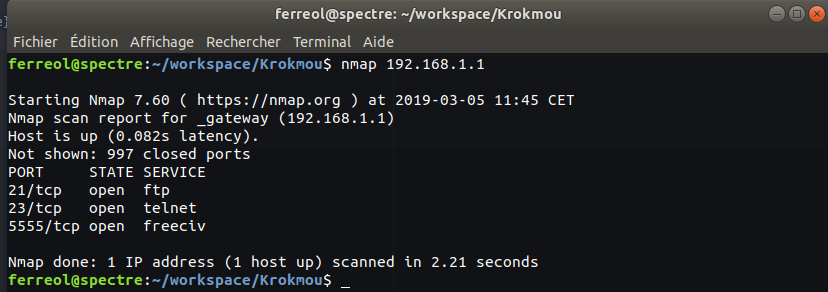
\includegraphics[scale=0.5]{images/scan_drone}
  \caption{Services disponibles sur le drone}
\end{figure}

La solution la plus simple serait de supprimer ces deux services et de les remplacer par un seul et même service, le service \textbf{SSH}. En effet, celui-ci combine l'aspect transfert de fichier de \textbf{FTP} et l'accès à distance de \textbf{Telnet} en plus d'offrir des garanties de sécurité avec notamment la présence d'un authentification à la connexion. Attention cependant, cette solution n'est viable que si le mot de passe par défault est changé à la première utilisation du drone.
